% Exploration map (generated by route/make_exploration_map_tex.py). Included from ai_workflow.tex.
\begin{figure}[H]
\centering
\resizebox{\textwidth}{!}{%
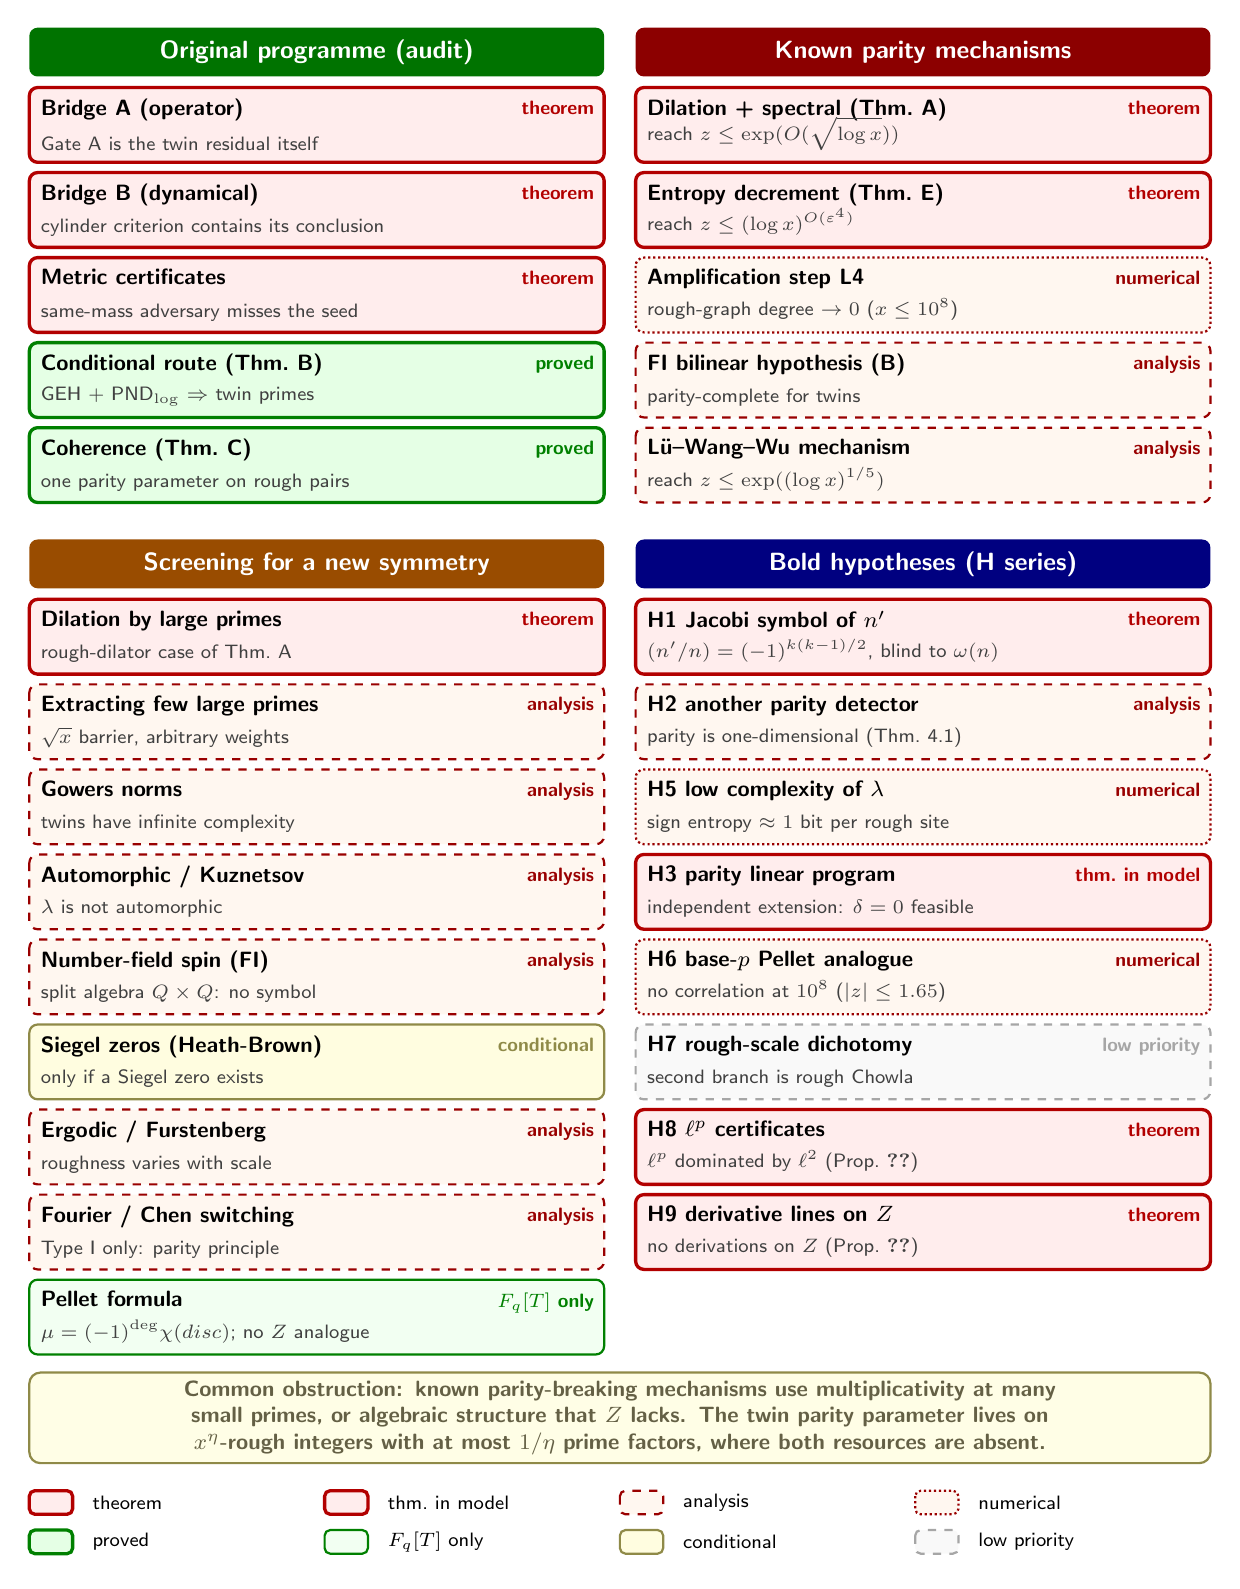
\begin{tikzpicture}[font=\sffamily]
\node[fill=green!45!black, text=white, minimum width=7.3cm, minimum height=0.62cm, inner xsep=0pt, outer sep=0pt, rounded corners=3pt, font=\small\bfseries\sffamily] at (3.650,0.450) {Original programme (audit)};
\draw[very thick, draw=red!70!black, fill=red!7, rounded corners=3pt] (0.000,0.000) rectangle (7.300,-0.950);
\node[anchor=north west, font=\footnotesize\bfseries\sffamily, inner sep=0pt] at (0.140,-0.140) {Bridge A (operator)};
\node[anchor=north east, font=\scriptsize\bfseries\sffamily, text=red!70!black, inner sep=0pt] at (7.180,-0.160) {theorem};
\node[anchor=south west, font=\scriptsize\sffamily, text=black!75, inner sep=0pt] at (0.140,-0.810) {Gate A is the twin residual itself};
\draw[very thick, draw=red!70!black, fill=red!7, rounded corners=3pt] (0.000,-1.080) rectangle (7.300,-2.030);
\node[anchor=north west, font=\footnotesize\bfseries\sffamily, inner sep=0pt] at (0.140,-1.220) {Bridge B (dynamical)};
\node[anchor=north east, font=\scriptsize\bfseries\sffamily, text=red!70!black, inner sep=0pt] at (7.180,-1.240) {theorem};
\node[anchor=south west, font=\scriptsize\sffamily, text=black!75, inner sep=0pt] at (0.140,-1.890) {cylinder criterion contains its conclusion};
\draw[very thick, draw=red!70!black, fill=red!7, rounded corners=3pt] (0.000,-2.160) rectangle (7.300,-3.110);
\node[anchor=north west, font=\footnotesize\bfseries\sffamily, inner sep=0pt] at (0.140,-2.300) {Metric certificates};
\node[anchor=north east, font=\scriptsize\bfseries\sffamily, text=red!70!black, inner sep=0pt] at (7.180,-2.320) {theorem};
\node[anchor=south west, font=\scriptsize\sffamily, text=black!75, inner sep=0pt] at (0.140,-2.970) {same-mass adversary misses the seed};
\draw[very thick, draw=green!50!black, fill=green!10, rounded corners=3pt] (0.000,-3.240) rectangle (7.300,-4.190);
\node[anchor=north west, font=\footnotesize\bfseries\sffamily, inner sep=0pt] at (0.140,-3.380) {Conditional route (Thm.~B)};
\node[anchor=north east, font=\scriptsize\bfseries\sffamily, text=green!50!black, inner sep=0pt] at (7.180,-3.400) {proved};
\node[anchor=south west, font=\scriptsize\sffamily, text=black!75, inner sep=0pt] at (0.140,-4.050) {GEH + PND$_{\log}$ $\Rightarrow$ twin primes};
\draw[very thick, draw=green!50!black, fill=green!10, rounded corners=3pt] (0.000,-4.320) rectangle (7.300,-5.270);
\node[anchor=north west, font=\footnotesize\bfseries\sffamily, inner sep=0pt] at (0.140,-4.460) {Coherence (Thm.~C)};
\node[anchor=north east, font=\scriptsize\bfseries\sffamily, text=green!50!black, inner sep=0pt] at (7.180,-4.480) {proved};
\node[anchor=south west, font=\scriptsize\sffamily, text=black!75, inner sep=0pt] at (0.140,-5.130) {one parity parameter on rough pairs};
\node[fill=red!55!black, text=white, minimum width=7.3cm, minimum height=0.62cm, inner xsep=0pt, outer sep=0pt, rounded corners=3pt, font=\small\bfseries\sffamily] at (11.350,0.450) {Known parity mechanisms};
\draw[very thick, draw=red!70!black, fill=red!7, rounded corners=3pt] (7.700,0.000) rectangle (15.000,-0.950);
\node[anchor=north west, font=\footnotesize\bfseries\sffamily, inner sep=0pt] at (7.840,-0.140) {Dilation + spectral (Thm.~A)};
\node[anchor=north east, font=\scriptsize\bfseries\sffamily, text=red!70!black, inner sep=0pt] at (14.880,-0.160) {theorem};
\node[anchor=south west, font=\scriptsize\sffamily, text=black!75, inner sep=0pt] at (7.840,-0.810) {reach $z\le\exp(O(\sqrt{\log x}))$};
\draw[very thick, draw=red!70!black, fill=red!7, rounded corners=3pt] (7.700,-1.080) rectangle (15.000,-2.030);
\node[anchor=north west, font=\footnotesize\bfseries\sffamily, inner sep=0pt] at (7.840,-1.220) {Entropy decrement (Thm.~E)};
\node[anchor=north east, font=\scriptsize\bfseries\sffamily, text=red!70!black, inner sep=0pt] at (14.880,-1.240) {theorem};
\node[anchor=south west, font=\scriptsize\sffamily, text=black!75, inner sep=0pt] at (7.840,-1.890) {reach $z\le(\log x)^{O(\varepsilon^4)}$};
\draw[thick, densely dotted, draw=red!60!black, fill=orange!6, rounded corners=3pt] (7.700,-2.160) rectangle (15.000,-3.110);
\node[anchor=north west, font=\footnotesize\bfseries\sffamily, inner sep=0pt] at (7.840,-2.300) {Amplification step L4};
\node[anchor=north east, font=\scriptsize\bfseries\sffamily, text=red!60!black, inner sep=0pt] at (14.880,-2.320) {numerical};
\node[anchor=south west, font=\scriptsize\sffamily, text=black!75, inner sep=0pt] at (7.840,-2.970) {rough-graph degree $\to0$ ($x\le10^8$)};
\draw[thick, dashed, draw=red!60!black, fill=orange!6, rounded corners=3pt] (7.700,-3.240) rectangle (15.000,-4.190);
\node[anchor=north west, font=\footnotesize\bfseries\sffamily, inner sep=0pt] at (7.840,-3.380) {FI bilinear hypothesis (B)};
\node[anchor=north east, font=\scriptsize\bfseries\sffamily, text=red!60!black, inner sep=0pt] at (14.880,-3.400) {analysis};
\node[anchor=south west, font=\scriptsize\sffamily, text=black!75, inner sep=0pt] at (7.840,-4.050) {parity-complete for twins};
\draw[thick, dashed, draw=red!60!black, fill=orange!6, rounded corners=3pt] (7.700,-4.320) rectangle (15.000,-5.270);
\node[anchor=north west, font=\footnotesize\bfseries\sffamily, inner sep=0pt] at (7.840,-4.460) {L\"u--Wang--Wu mechanism};
\node[anchor=north east, font=\scriptsize\bfseries\sffamily, text=red!60!black, inner sep=0pt] at (14.880,-4.480) {analysis};
\node[anchor=south west, font=\scriptsize\sffamily, text=black!75, inner sep=0pt] at (7.840,-5.130) {reach $z\le\exp((\log x)^{1/5})$};
\node[fill=orange!60!black, text=white, minimum width=7.3cm, minimum height=0.62cm, inner xsep=0pt, outer sep=0pt, rounded corners=3pt, font=\small\bfseries\sffamily] at (3.650,-6.050) {Screening for a new symmetry};
\draw[very thick, draw=red!70!black, fill=red!7, rounded corners=3pt] (0.000,-6.500) rectangle (7.300,-7.450);
\node[anchor=north west, font=\footnotesize\bfseries\sffamily, inner sep=0pt] at (0.140,-6.640) {Dilation by large primes};
\node[anchor=north east, font=\scriptsize\bfseries\sffamily, text=red!70!black, inner sep=0pt] at (7.180,-6.660) {theorem};
\node[anchor=south west, font=\scriptsize\sffamily, text=black!75, inner sep=0pt] at (0.140,-7.310) {rough-dilator case of Thm.~A};
\draw[thick, dashed, draw=red!60!black, fill=orange!6, rounded corners=3pt] (0.000,-7.580) rectangle (7.300,-8.530);
\node[anchor=north west, font=\footnotesize\bfseries\sffamily, inner sep=0pt] at (0.140,-7.720) {Extracting few large primes};
\node[anchor=north east, font=\scriptsize\bfseries\sffamily, text=red!60!black, inner sep=0pt] at (7.180,-7.740) {analysis};
\node[anchor=south west, font=\scriptsize\sffamily, text=black!75, inner sep=0pt] at (0.140,-8.390) {$\sqrt x$ barrier, arbitrary weights};
\draw[thick, dashed, draw=red!60!black, fill=orange!6, rounded corners=3pt] (0.000,-8.660) rectangle (7.300,-9.610);
\node[anchor=north west, font=\footnotesize\bfseries\sffamily, inner sep=0pt] at (0.140,-8.800) {Gowers norms};
\node[anchor=north east, font=\scriptsize\bfseries\sffamily, text=red!60!black, inner sep=0pt] at (7.180,-8.820) {analysis};
\node[anchor=south west, font=\scriptsize\sffamily, text=black!75, inner sep=0pt] at (0.140,-9.470) {twins have infinite complexity};
\draw[thick, dashed, draw=red!60!black, fill=orange!6, rounded corners=3pt] (0.000,-9.740) rectangle (7.300,-10.690);
\node[anchor=north west, font=\footnotesize\bfseries\sffamily, inner sep=0pt] at (0.140,-9.880) {Automorphic / Kuznetsov};
\node[anchor=north east, font=\scriptsize\bfseries\sffamily, text=red!60!black, inner sep=0pt] at (7.180,-9.900) {analysis};
\node[anchor=south west, font=\scriptsize\sffamily, text=black!75, inner sep=0pt] at (0.140,-10.550) {$\lambda$ is not automorphic};
\draw[thick, dashed, draw=red!60!black, fill=orange!6, rounded corners=3pt] (0.000,-10.820) rectangle (7.300,-11.770);
\node[anchor=north west, font=\footnotesize\bfseries\sffamily, inner sep=0pt] at (0.140,-10.960) {Number-field spin (FI)};
\node[anchor=north east, font=\scriptsize\bfseries\sffamily, text=red!60!black, inner sep=0pt] at (7.180,-10.980) {analysis};
\node[anchor=south west, font=\scriptsize\sffamily, text=black!75, inner sep=0pt] at (0.140,-11.630) {split algebra $\mathbb Q\times\mathbb Q$: no symbol};
\draw[thick, draw=yellow!50!black, fill=yellow!12, rounded corners=3pt] (0.000,-11.900) rectangle (7.300,-12.850);
\node[anchor=north west, font=\footnotesize\bfseries\sffamily, inner sep=0pt] at (0.140,-12.040) {Siegel zeros (Heath-Brown)};
\node[anchor=north east, font=\scriptsize\bfseries\sffamily, text=yellow!50!black, inner sep=0pt] at (7.180,-12.060) {conditional};
\node[anchor=south west, font=\scriptsize\sffamily, text=black!75, inner sep=0pt] at (0.140,-12.710) {only if a Siegel zero exists};
\draw[thick, dashed, draw=red!60!black, fill=orange!6, rounded corners=3pt] (0.000,-12.980) rectangle (7.300,-13.930);
\node[anchor=north west, font=\footnotesize\bfseries\sffamily, inner sep=0pt] at (0.140,-13.120) {Ergodic / Furstenberg};
\node[anchor=north east, font=\scriptsize\bfseries\sffamily, text=red!60!black, inner sep=0pt] at (7.180,-13.140) {analysis};
\node[anchor=south west, font=\scriptsize\sffamily, text=black!75, inner sep=0pt] at (0.140,-13.790) {roughness varies with scale};
\draw[thick, dashed, draw=red!60!black, fill=orange!6, rounded corners=3pt] (0.000,-14.060) rectangle (7.300,-15.010);
\node[anchor=north west, font=\footnotesize\bfseries\sffamily, inner sep=0pt] at (0.140,-14.200) {Fourier / Chen switching};
\node[anchor=north east, font=\scriptsize\bfseries\sffamily, text=red!60!black, inner sep=0pt] at (7.180,-14.220) {analysis};
\node[anchor=south west, font=\scriptsize\sffamily, text=black!75, inner sep=0pt] at (0.140,-14.870) {Type I only: parity principle};
\draw[thick, draw=green!50!black, fill=green!5, rounded corners=3pt] (0.000,-15.140) rectangle (7.300,-16.090);
\node[anchor=north west, font=\footnotesize\bfseries\sffamily, inner sep=0pt] at (0.140,-15.280) {Pellet formula};
\node[anchor=north east, font=\scriptsize\bfseries\sffamily, text=green!50!black, inner sep=0pt] at (7.180,-15.300) {$\mathbb F_q[T]$ only};
\node[anchor=south west, font=\scriptsize\sffamily, text=black!75, inner sep=0pt] at (0.140,-15.950) {$\mu=(-1)^{\deg}\chi(\operatorname{disc})$; no $\mathbb Z$ analogue};
\node[fill=blue!50!black, text=white, minimum width=7.3cm, minimum height=0.62cm, inner xsep=0pt, outer sep=0pt, rounded corners=3pt, font=\small\bfseries\sffamily] at (11.350,-6.050) {Bold hypotheses (H series)};
\draw[very thick, draw=red!70!black, fill=red!7, rounded corners=3pt] (7.700,-6.500) rectangle (15.000,-7.450);
\node[anchor=north west, font=\footnotesize\bfseries\sffamily, inner sep=0pt] at (7.840,-6.640) {H1 Jacobi symbol of $n'$};
\node[anchor=north east, font=\scriptsize\bfseries\sffamily, text=red!70!black, inner sep=0pt] at (14.880,-6.660) {theorem};
\node[anchor=south west, font=\scriptsize\sffamily, text=black!75, inner sep=0pt] at (7.840,-7.310) {$(n'/n)=(-1)^{k(k-1)/2}$, blind to $\omega(n)$};
\draw[thick, dashed, draw=red!60!black, fill=orange!6, rounded corners=3pt] (7.700,-7.580) rectangle (15.000,-8.530);
\node[anchor=north west, font=\footnotesize\bfseries\sffamily, inner sep=0pt] at (7.840,-7.720) {H2 another parity detector};
\node[anchor=north east, font=\scriptsize\bfseries\sffamily, text=red!60!black, inner sep=0pt] at (14.880,-7.740) {analysis};
\node[anchor=south west, font=\scriptsize\sffamily, text=black!75, inner sep=0pt] at (7.840,-8.390) {parity is one-dimensional (Thm.~4.1)};
\draw[thick, densely dotted, draw=red!60!black, fill=orange!6, rounded corners=3pt] (7.700,-8.660) rectangle (15.000,-9.610);
\node[anchor=north west, font=\footnotesize\bfseries\sffamily, inner sep=0pt] at (7.840,-8.800) {H5 low complexity of $\lambda$};
\node[anchor=north east, font=\scriptsize\bfseries\sffamily, text=red!60!black, inner sep=0pt] at (14.880,-8.820) {numerical};
\node[anchor=south west, font=\scriptsize\sffamily, text=black!75, inner sep=0pt] at (7.840,-9.470) {sign entropy $\approx1$ bit per rough site};
\draw[very thick, draw=red!70!black, fill=red!7, rounded corners=3pt] (7.700,-9.740) rectangle (15.000,-10.690);
\node[anchor=north west, font=\footnotesize\bfseries\sffamily, inner sep=0pt] at (7.840,-9.880) {H3 parity linear program};
\node[anchor=north east, font=\scriptsize\bfseries\sffamily, text=red!70!black, inner sep=0pt] at (14.880,-9.900) {thm.\ in model};
\node[anchor=south west, font=\scriptsize\sffamily, text=black!75, inner sep=0pt] at (7.840,-10.550) {independent extension: $\delta=0$ feasible};
\draw[thick, densely dotted, draw=red!60!black, fill=orange!6, rounded corners=3pt] (7.700,-10.820) rectangle (15.000,-11.770);
\node[anchor=north west, font=\footnotesize\bfseries\sffamily, inner sep=0pt] at (7.840,-10.960) {H6 base-$p$ Pellet analogue};
\node[anchor=north east, font=\scriptsize\bfseries\sffamily, text=red!60!black, inner sep=0pt] at (14.880,-10.980) {numerical};
\node[anchor=south west, font=\scriptsize\sffamily, text=black!75, inner sep=0pt] at (7.840,-11.630) {no correlation at $10^8$ ($|z|\le1.65$)};
\draw[thick, dashed, draw=gray!70, fill=gray!5, rounded corners=3pt] (7.700,-11.900) rectangle (15.000,-12.850);
\node[anchor=north west, font=\footnotesize\bfseries\sffamily, inner sep=0pt] at (7.840,-12.040) {H7 rough-scale dichotomy};
\node[anchor=north east, font=\scriptsize\bfseries\sffamily, text=gray!70, inner sep=0pt] at (14.880,-12.060) {low priority};
\node[anchor=south west, font=\scriptsize\sffamily, text=black!75, inner sep=0pt] at (7.840,-12.710) {second branch is rough Chowla};
\draw[very thick, draw=red!70!black, fill=red!7, rounded corners=3pt] (7.700,-12.980) rectangle (15.000,-13.930);
\node[anchor=north west, font=\footnotesize\bfseries\sffamily, inner sep=0pt] at (7.840,-13.120) {H8 $\ell^p$ certificates};
\node[anchor=north east, font=\scriptsize\bfseries\sffamily, text=red!70!black, inner sep=0pt] at (14.880,-13.140) {theorem};
\node[anchor=south west, font=\scriptsize\sffamily, text=black!75, inner sep=0pt] at (7.840,-13.790) {$\ell^p$ dominated by $\ell^2$ (Prop.~\ref{prop:L})};
\draw[very thick, draw=red!70!black, fill=red!7, rounded corners=3pt] (7.700,-14.060) rectangle (15.000,-15.010);
\node[anchor=north west, font=\footnotesize\bfseries\sffamily, inner sep=0pt] at (7.840,-14.200) {H9 derivative lines on $\mathbb Z$};
\node[anchor=north east, font=\scriptsize\bfseries\sffamily, text=red!70!black, inner sep=0pt] at (14.880,-14.220) {theorem};
\node[anchor=south west, font=\scriptsize\sffamily, text=black!75, inner sep=0pt] at (7.840,-14.870) {no derivations on $\mathbb Z$ (Prop.~\ref{prop:noderiv})};
\draw[thick, draw=yellow!50!black, fill=yellow!10, rounded corners=4pt] (0,-16.320) rectangle (15.000,-17.470);
\node[align=center, text width=14.60cm, font=\footnotesize\bfseries\sffamily, text=yellow!30!black] at (7.500,-16.895) {Common obstruction: known parity-breaking mechanisms use multiplicativity at many small primes, or algebraic structure that $\mathbb Z$ lacks. The twin parity parameter lives on $x^\eta$-rough integers with at most $1/\eta$ prime factors, where both resources are absent.};
\draw[very thick, draw=red!70!black, fill=red!7, rounded corners=2pt] (0.000,-17.820) rectangle (0.550,-18.120);
\node[anchor=west, font=\scriptsize\sffamily] at (0.680,-17.970) {theorem};
\draw[very thick, draw=red!70!black, fill=red!7, rounded corners=2pt] (3.750,-17.820) rectangle (4.300,-18.120);
\node[anchor=west, font=\scriptsize\sffamily] at (4.430,-17.970) {thm.\ in model};
\draw[thick, dashed, draw=red!60!black, fill=orange!6, rounded corners=2pt] (7.500,-17.820) rectangle (8.050,-18.120);
\node[anchor=west, font=\scriptsize\sffamily] at (8.180,-17.970) {analysis};
\draw[thick, densely dotted, draw=red!60!black, fill=orange!6, rounded corners=2pt] (11.250,-17.820) rectangle (11.800,-18.120);
\node[anchor=west, font=\scriptsize\sffamily] at (11.930,-17.970) {numerical};
\draw[very thick, draw=green!50!black, fill=green!10, rounded corners=2pt] (0.000,-18.320) rectangle (0.550,-18.620);
\node[anchor=west, font=\scriptsize\sffamily] at (0.680,-18.470) {proved};
\draw[thick, draw=green!50!black, fill=green!5, rounded corners=2pt] (3.750,-18.320) rectangle (4.300,-18.620);
\node[anchor=west, font=\scriptsize\sffamily] at (4.430,-18.470) {$\mathbb F_q[T]$ only};
\draw[thick, draw=yellow!50!black, fill=yellow!12, rounded corners=2pt] (7.500,-18.320) rectangle (8.050,-18.620);
\node[anchor=west, font=\scriptsize\sffamily] at (8.180,-18.470) {conditional};
\draw[thick, dashed, draw=gray!70, fill=gray!5, rounded corners=2pt] (11.250,-18.320) rectangle (11.800,-18.620);
\node[anchor=west, font=\scriptsize\sffamily] at (11.930,-18.470) {low priority};
\end{tikzpicture}}
\caption{Map of every route explored in this project, with its status. ``Theorem'' means a complete proof in this paper or in the separate audit of the original programme (first column); ``thm.\ in model'' means an explicit construction that is rigorous within the stated model; ``analysis'' and ``numerical'' are judgements about specific arguments or data, not theorems. All entries were obtained with AI assistance and have not yet been checked by a specialist (Appendix~\ref{app:ai}).}
\label{fig:exploration}
\end{figure}
